%% WMG.draft.tex
%% Windowed Minority Guidance: Timestep-Localized Effects in Diffusion
%% Denoising Across a Six-Scale Guidance Sweep
%% Vittoria Lanzo — 2026
%% Expanded report: original scale=1.0 abstract + multi-scale sweep,
%% sliding window, and robustness sections. Single-column 10pt, ~6 pages.

\documentclass[10pt]{article}

\usepackage{times}
\usepackage{amsmath}
\usepackage{amssymb}
\usepackage{booktabs}
\usepackage{hyperref}
\usepackage{microtype}
\usepackage{geometry}
\usepackage{listings}
\usepackage{xcolor}
\usepackage{multirow}
\usepackage{caption}
\usepackage{graphicx}

\geometry{
  letterpaper,
  top=1in, bottom=1in,
  left=1in, right=1in
}

\hypersetup{
  colorlinks=true,
  linkcolor=blue!70!black,
  citecolor=blue!70!black,
  urlcolor=blue!70!black
}

\lstset{
  basicstyle=\small\ttfamily,
  breaklines=true,
  frame=single,
  numbers=left,
  numberstyle=\tiny,
  xleftmargin=1.5em,
  framexleftmargin=1.5em
}

% -----------------------------------------------------------------------
\title{\textbf{Windowed Minority Guidance: Timestep-Localized Effects in
Diffusion Denoising Across a Six-Scale Guidance Sweep}}

\author{%
  Vittoria Lanzo \\
  \textit{Independent Researcher}
}

\date{}
% -----------------------------------------------------------------------

\begin{document}

\maketitle

% -----------------------------------------------------------------------
\begin{abstract}
Minority guidance~\cite{um2024minority} steers diffusion sampling toward
under-represented data regions via a classifier gradient at every denoising
step.  We test whether this effect is timestep-localized, comparing three
equal-thirds windows named by timestep index (not DDPM chronological order):
early $t\!\in\![0,333)$ (low noise, fine-detail refinement),
mid $t\!\in\![333,667)$, late $t\!\in\![667,1000)$ (high noise, coarse-structure
formation)---against full-chain and no-guidance baselines over 50 seeds on LSUN
Bedroom, repeated across six guidance scales $s\in\{0.5,1.0,2.0,3.5,5.0,7.0\}$
(including Um et al.'s operating scale $s=3.5$;
1500 runs in the sweep, plus a sliding-window and a replication study).  The
mid window has the largest single-window relative effect at every scale
(increasing across the sweep from $\Delta_\mathrm{rel}=0.456$ at $s=0.5$ to
$0.832$ at $s=7.0$, after a near-flat $s\!\le\!1.0$ segment), and the early
window achieves lower classifier loss than baseline
on all 50 seeds at every scale ($W=0$, $r_\mathrm{rb}=1.000$; one sample per
seed, with modest per-seed magnitude---pooled Cohen's $d=0.14$ at $s=0.5$, growing
with scale).  The late-window effect is not
significant under the per-scale Bonferroni threshold $\alpha/7=0.00714$ for
$s\le 1.0$ but is significant from $s=2.0$ upward; mid's advantage over the
late window is likewise significant only for $s\ge2.0$ (at $s\le1.0$ the two
are statistically indistinguishable), and the late-vs-early
difference is never significant.  A 250-step sliding window at $s=3.5$ peaks
at $t\!\in\![375,625)$ with a unimodal profile.  The mid $\Delta_\mathrm{rel}$
matches on independent seeds 51--100 ($0.693$ vs.\ $0.693$), though both
baseline and mid means shifted ($11.978\to12.759$ and $4.31\to4.60$
respectively), so the match reflects similarly-shifted numerator and denominator
rather than absolute-effect reproduction.
The relative-effect comparison across scales is partly denominator-sensitive
(the full-chain mean loss approaches zero as $s$ rises, making the denominator
$(\text{baseline}-\overline{\text{full}})$ grow, with ratio instability worst
at low $s$) and is association, not a causal decomposition; results are a
single dataset, architecture, one sample per seed, and classifier loss is a
proxy rather than a perceptual metric.
\end{abstract}

% -----------------------------------------------------------------------
\section{Introduction}
\label{sec:intro}

Classifier-guided diffusion models~\cite{dhariwal2021diffusion} steer generation
with classifier gradients at every denoising step.  Um et al.\ \cite{um2024minority}
extend this to \emph{minority guidance}, directing sampling toward underrepresented
data regions.  Because decreasing timesteps transition from coarse-structure formation to
fine-detail refinement~\cite{ho2020ddpm}, the mid-chain phase may be most receptive to
minority gradient signals---enabling cheaper inference-time guidance if guidance
there recovers most of the full-chain effect.  Kynk\"{a}\"{a}nniemi et al.\
\cite{kynkaanniemi2024interval} recently showed that classifier-free guidance
(CFG) applied only in a middle interval improves FID on class-conditional
ImageNet, with guidance harmful at high noise and unnecessary at low noise.
We investigate whether an analogous localization holds for the minority
\emph{classifier} guidance of Um et al., which operates via an external
minority-score signal rather than a conditional score gap.  We test this directly: the
original single-scale experiment~\cite{lanzo2026windowed} (Section~\ref{sec:results}) reported findings
that partially challenge it, and its stated limitation was that results might not
generalize to other scales.  This report addresses that limitation directly,
repeating the five-condition experiment across six guidance scales
(Section~\ref{sec:sweep}), refining the window granularity with a sliding window
(Section~\ref{sec:sliding}), and probing sample-size and seed robustness
(Section~\ref{sec:robustness}).

% -----------------------------------------------------------------------
\section{Experiment}
\label{sec:experiment}

We use the LSUN Bedroom 256$\times$256 diffusion model with the frozen minority
classifier of Um et al.~\cite{um2024minority} (\texttt{mc\_lsun.pt}) stacked on
top of OpenAI's ImageNet feature extractor (\texttt{256x256\_classifier.pt}),
\texttt{timestep\_respacing=250}.
\textbf{Class 99:} Um et al.\ assign images to 100 ordinal minority-score
buckets; class~99 is the rarest (most minority) bucket, not a semantic label.  Five conditions:
\emph{baseline}, \emph{minority-full} $t\!\in\![0,1000)$, \emph{minority-early}
$t\!\in\![0,333)$, \emph{minority-mid} $t\!\in\![333,667)$, \emph{minority-late}
$t\!\in\![667,1000)$.  Guidance is rescaled to the active window only; results
may not generalize.  The original experiment ran 50 seeds $\times$ 5 conditions
= 250 runs at \texttt{guidance\_scale=1.0} (Kaggle P100, float32).  Seeds
$1$--$10$ used for protocol verification (no systematic bias observed); the
remaining seeds follow the same configuration, which is based on the protocol,
checkpoints, and class-id of Um et al.~\cite{um2024minority}.

\textbf{Sweep extension.}  To examine scale sensitivity, the same five-condition
protocol is repeated at five additional scales
$s\in\{0.5,2.0,3.5,5.0,7.0\}$, each 50 seeds $\times$ 5 conditions, and combined
with the original $s=1.0$ run for a six-scale sweep
($s\in\{0.5,1.0,2.0,3.5,5.0,7.0\}$).  The five new scales were chosen to bracket
Um et al.'s released LSUN Bedroom sampling configuration ($s=3.5$) on both sides; this scale set
was fixed before the sweep was run and was not adapted to the results.
\textbf{Shared baseline:} the same 50 seeds at \texttt{guidance\_scale=0} serve
as baseline for all six scales; cross-scale comparisons are between
\emph{within-scale} condition pairs, not across baselines.

\textbf{Primary metric}: classifier cross-entropy loss at class 99 (lower =
stronger guidance).  Softmax confidence is corroborated only---at $s=1.0$ the
single-scale confidence distributions are severely right-skewed (mean/median:
full 108x; late 154x; mid 46x; early 58x).  Switching from the originally planned metric (classifier confidence) to loss is an
unplanned procedural deviation; classifier-based effect sizes are one order of
magnitude smaller.

\paragraph{Timestep convention.}
Window names follow the \emph{numerical magnitude of the timestep
index~$t$}, not the chronological order of the DDPM reverse
process~\cite{ho2020ddpm}.  ``Early'' ($t\!\in\![0,333)$) therefore
corresponds to \emph{low-noise} timesteps (fine-detail refinement);
``late'' ($t\!\in\![667,1000)$) to \emph{high-noise} timesteps
(coarse-structure formation).

\paragraph{Windowed \texttt{cond\_fn}.}
Guidance is applied exclusively within the designated timestep window.
Outside the window, the \texttt{cond\_fn} is a no-op, returning a zero tensor.  Full details are given in Appendix~\ref{sec:implementation}.

% -----------------------------------------------------------------------
\section{Results: Single Scale ($s=1.0$)}
\label{sec:results}

\textbf{Table~\ref{tab:conditions}} ($n=50$; lower loss = stronger guidance).

\begin{table}[h]
\centering
\caption{Condition statistics ($n=50$ seeds; scale $= 1.0$; LSUN Bedroom).
Lower mean loss indicates stronger minority-class guidance.
Win Rate is the fraction of seeds on which the condition beats baseline.
Relative Effect $= (\text{baseline} - \overline{\text{cond}}) /
(\text{baseline} - \overline{\text{full}})$;
not a causal decomposition (windows interact across the rejection trajectory).}
\label{tab:conditions}
\renewcommand{\arraystretch}{1.1}
\begin{tabular}{@{}lcccc@{}}
\toprule
\textbf{Condition} & \textbf{Mean Loss} & \textbf{CV} &
  \textbf{Win Rate} & \textbf{Relative Effect} \\
\midrule
baseline        & 11.978 & 0.19 & ---   & 0.000 \\
minority-early  & 11.129 & 0.23 & 50/50 & 0.162 \\
minority-mid    &  9.591 & 0.35 & 39/50 & 0.456 \\
minority-late   & 10.717 & 0.30 & 34/50 & 0.241 \\
minority-full   &  6.741 & 0.61 & 44/50 & 1.000 \\
\bottomrule
\end{tabular}
\end{table}

The rank ordering mid $>$ late $>$ early $>$ baseline holds across 50 seeds
($r_\mathrm{rb} = 1.000, 0.812, 0.432, 0.925$ for early, mid, late, full
vs.\ baseline respectively).  \textbf{Table~\ref{tab:wilcoxon}} reports
Wilcoxon signed-rank tests, Bonferroni threshold $\alpha/7 = 0.00714$.

\begin{table}[h]
\centering
\caption{Wilcoxon signed-rank tests ($n=50$ pairs; two-sided; \texttt{zero\_method=zsplit}).
$r_\mathrm{rb} \in [0,1]$: rank-biserial correlation (effect size);
$r_\mathrm{rb} > 0$ indicates first condition has lower loss.
Survives Bonferroni correction if $p < \alpha/7 = 0.00714$.
The family of seven comprises the four window-vs-baseline comparisons plus the
three cross-window pairs (mid-vs-late, late-vs-early, full-vs-mid) that directly
bear on the localization claim; the three remaining pairs (full-vs-early,
full-vs-late, mid-vs-early) compare conditions with well-established ordering
and were excluded from the pre-specified family.}
\label{tab:wilcoxon}
\renewcommand{\arraystretch}{1.1}
\begin{tabular}{@{}llcc@{}}
\toprule
\textbf{Comparison} & \textbf{W} & \textbf{$p$-value} & \textbf{$r_\mathrm{rb}$} \\
\midrule
mid vs.\ baseline   & 120  & $<0.0001$ & 0.812 \\
late vs.\ baseline  & 362  & $0.00716$ & 0.432 \\
early vs.\ baseline &   0  & $<0.0001$ & 1.000 \\
full vs.\ baseline  &  48  & $<0.0001$ & 0.925 \\
mid vs.\ late       & 391  & $0.0166$  & 0.387 \\
late vs.\ early     & 547  & $0.3882$  & 0.142 \\
full vs.\ mid       & 181  & $<0.0001$ & 0.716 \\
\bottomrule
\end{tabular}
\end{table}

Mid recovers 0.456 of full-chain loss reduction (mean 9.591 vs.\ baseline
11.978 and full 6.741).  Analysis criterion: Bonferroni-corrected $p < \alpha/7 = 0.00714$.
Bootstrap 95\% CI on mid mean: [8.67, 10.50].  The relative effect
($\Delta_\mathrm{rel} = 0.456$) measures fraction of full-chain loss
reduction recovered; the CI bounds are absolute loss units and are not
directly comparable to $\Delta_\mathrm{rel}$.

\medskip

\noindent\textbf{Key finding}: at $s=1.0$, early-window guidance (operating at
low noise, fine-detail phase) reduces classifier loss on all 50 seeds
($W = 0$, $r_\mathrm{rb} = 1.000$, $p < 0.0001$); confidence corroborates this
direction only.  We measured no perceptual or quality metric, so this is a
statement about the classifier-loss objective, not about minority-class image
quality, and we draw no causal conclusion.

\medskip

\noindent\textbf{Late vs.\ Early at scale$=1.0$}: the coarse-structure (late)
window has a higher $\Delta_\mathrm{rel}$ point estimate than the fine-detail
(early) window at this scale, though the difference is not statistically
significant ($p = 0.388$).

% -----------------------------------------------------------------------
\section{Results: Multi-Scale Sweep}
\label{sec:sweep}

We repeat the five-condition experiment across six guidance scales
$s\in\{0.5,1.0,2.0,3.5,5.0,7.0\}$ (50 seeds each).
\textbf{Table~\ref{tab:crossscale}} reports the cross-scale relative-effect
matrix and \textbf{Figure~\ref{fig:releffects}} plots $\Delta_\mathrm{rel}$
against scale for each window.  Three patterns hold across the sweep: the mid
window has the largest single-window relative effect at every scale; the early
window beats baseline on all 50 seeds at every scale; and the late window
becomes significant only from $s=2.0$ upward.

\begin{table}[h]
\centering
\caption{Cross-scale relative-effect matrix
($\Delta_\mathrm{rel} = (\text{baseline}-\overline{\text{cond}})/
(\text{baseline}-\overline{\text{full}})$; $n=50$ seeds per scale; LSUN
Bedroom).  The full condition is $1.000$ by construction at every scale.
Last column: 95\% bootstrap CI on the mid \emph{mean loss} (absolute units;
independent-sample resampling of mid losses, 10{,}000 resamples, \texttt{random.seed(42)};
not directly comparable to the $\Delta_\mathrm{rel}$ CIs in Figure~\ref{fig:releffects},
which use paired-seed resampling of $\Delta_\mathrm{rel}$ via \texttt{np.random.default\_rng(42)}).}
\label{tab:crossscale}
\renewcommand{\arraystretch}{1.1}
\begin{tabular}{@{}lcccc@{}}
\toprule
\textbf{Scale $s$} & \textbf{early} & \textbf{mid} & \textbf{late} &
  \textbf{mid mean-loss CI} \\
\midrule
0.5 & 0.176 & 0.456 & 0.149 & [10.37, 11.81] \\
1.0 & 0.162 & 0.456 & 0.241 & [8.67, 10.50] \\
2.0 & 0.242 & 0.544 & 0.294 & [5.82, 8.02] \\
3.5 & 0.379 & 0.693 & 0.405 & [3.28, 5.41] \\
5.0 & 0.494 & 0.774 & 0.500 & [2.13, 4.04] \\
7.0 & 0.608 & 0.832 & 0.566 & [1.40, 3.24] \\
\bottomrule
\end{tabular}
\end{table}

\begin{figure}[h]
\centering

\includegraphics[width=0.78\linewidth]{fig1_relative_effects.pdf}
\caption{Relative effect $\Delta_\mathrm{rel}$ versus guidance scale $s$ for
the early, mid, and late windows.  Mid has the largest relative effect at every
scale; early and late
track each other closely and are never significantly different (late-vs-early
$p\ge0.357$ at every scale, minimum at $s=2.0$), with overlapping CIs throughout,
so the apparent changes in their relative ordering across scales are not
statistically meaningful.
The $x$-axis is linear in $s$; error bars are 95\% bootstrap CIs on
$\Delta_\mathrm{rel}$ (paired-seed resampling, 10{,}000 resamples).  The
late-window CI at $s=0.5$ spans zero, consistent with its non-significance there.}
\label{fig:releffects}
\end{figure}

\paragraph{Mid-window relative effect is largest at every scale.}
The mid window's relative effect rises with scale (effectively flat between
$s=0.5$ and $s=1.0$, then increasing)---$0.456$
($s=0.5$), $0.456$ ($s=1.0$), $0.544$ ($s=2.0$), $0.693$ ($s=3.5$), $0.774$
($s=5.0$), $0.832$ ($s=7.0$)---and has the largest point estimate among the
three windows at every scale.  Mid vs.\ baseline survives the per-scale Bonferroni threshold
($\alpha/7=0.00714$) at all six scales (e.g.\ $W=120,\ p<0.0001$ at $s=1.0$;
$W=9,\ p<0.0001$ at $s=3.5$; $W=0,\ p<0.0001$ at $s=5.0$ and $s=7.0$).
Mid's lead over the \emph{late} window, however, is statistically significant
only for $s\ge2.0$ (mid-vs-late $p=9.9\times10^{-5}$ at $s=2.0$, down to
$1.4\times10^{-5}$ at $s=7.0$); at $s=0.5$ ($p=0.082$) and $s=1.0$ ($p=0.0166$,
failing $\alpha/7$) mid has the larger point estimate but its superiority over
the late window is not statistically established.  So mid-window ``dominance''
is a tested claim for $s\ge2.0$ and a point-estimate ordering at the two lowest
scales.  The
rising $\Delta_\mathrm{rel}$ should be read with care: because
$\Delta_\mathrm{rel}$ uses $(\text{baseline}-\overline{\text{full}})$ as its
denominator and the full-chain mean loss approaches $0$ as $s$ grows (full
mean $10.05$ at $s=0.5$ down to $0.281$ at $s=7.0$), the cross-scale
comparison is partly denominator-sensitive and is an association, not a causal
decomposition of where guidance acts.

\paragraph{Late-window significance transition.}
The late window does not survive the per-scale Bonferroni threshold for
$s\le 1.0$ (late vs.\ baseline $p=0.163$ at $s=0.5$; $p=0.00716$ at $s=1.0$,
narrowly above $\alpha/7=0.00714$) but is significant from $s=2.0$ upward
($p=4.03\times10^{-6}$ at $s=2.0$; $p=7.24\times10^{-10}$ at $s=3.5$;
$p<10^{-11}$ at $s=5.0$ and $s=7.0$).  The late-window relative effect rises
correspondingly from $0.149$ to $0.566$ across the sweep.

\paragraph{Early window: all seeds improve at every scale.}
The early window beats baseline on all 50 seeds (one sample per seed) at every
scale: early vs.\
baseline gives $W=0$, $r_\mathrm{rb}=1.000$, win rate $50/50$, $p<0.0001$ at
each of the six scales.  This is an extreme but consistently observed result
(all 50 paired differences favor the early window); we report it as the
observed win rate rather than interpreting it as a causal effect.  Per-seed reductions are reliable in direction but modest when measured as
pooled Cohen's $d$ ($d=0.14$ at $s=0.5$, growing with scale); the paired
$d_z$ (mean paired difference divided by its SD) is larger ($d_z=1.02$ at
$s=0.5$) because it removes between-seed variance shared across conditions.

\paragraph{Late vs.\ early is never significant.}
Across all six scales the late-vs-early comparison never survives Bonferroni
correction: $p=0.759$ ($s=0.5$), $0.388$ ($s=1.0$), $0.357$ ($s=2.0$), $0.585$
($s=3.5$), $0.992$ ($s=5.0$), $0.432$ ($s=7.0$).  The two windows track each
other closely (Figure~\ref{fig:releffects}): their $\Delta_\mathrm{rel}$ point
estimates change relative order across scales (early higher at $s=0.5$, late
higher through the mid scales, early higher again at $s=7.0$) and are nearly
equal at $s=5.0$ ($\Delta_\mathrm{rel}$: early $0.494$ vs.\ late $0.500$), but
with overlapping bootstrap CIs and no significant test at any scale, these
order changes are not evidence that one window outperforms the other.

\paragraph{Cross-scale multiple comparisons.}
The seven within-scale comparisons are corrected at $\alpha/7=0.00714$ as in
the single-scale analysis; this per-scale correction is unchanged by adding
scales.  Pooling the six scales raises a multiple-comparisons question across
the full $6\times7=42$ comparisons; under the stricter cross-scale threshold
$\alpha/42=0.00119$ the late-vs-baseline result at $s=1.0$ ($p=0.00716$) and at
$s=0.5$ ($p=0.163$) remain non-significant, while the mid-, early-, and
full-vs-baseline results and the late-vs-baseline results for $s\ge 2.0$
continue to pass.  This $\alpha/42$ family covers the main sweep's
$6\times7$ condition comparisons; the sliding-window is a separate localization
follow-up (corrected within itself at $\alpha/8$) and the sample-size sweep is a
post-hoc robustness probe (corrected at $\alpha/7$ within each $n$), rather than
folded into the sweep family.

% -----------------------------------------------------------------------
\section{Results: Sliding Window}
\label{sec:sliding}

To refine the three coarse equal-thirds windows, we sweep a 250-step window of
constant width across the chain at $s=3.5$---the operating scale of Um et
al.~\cite{um2024minority}---stepped by 125 raw timesteps
(\texttt{slide\_0}: $t\!\in\![0,250)$ through \texttt{slide\_6}:
$t\!\in\![750,1000)$; seven windows, 50 seeds each).  All seven sliding windows
beat baseline under a Bonferroni threshold computed for this experiment's eight
comparisons (seven windows plus full), $\alpha/8=0.00625$---separate from the
main sweep's $\alpha/7$.  The relative-effect profile is
\textbf{unimodal} (Figure~\ref{fig:sliding}), peaking at \texttt{slide\_3}
($t\!\in\![375,625)$) with $\Delta_\mathrm{rel}=0.536$ (mean loss $6.050$,
$W=8$, $p<0.0001$, $r_\mathrm{rb}=0.987$; Table~\ref{tab:sliding}).

\begin{table}[h]
\centering
\caption{Sliding-window results at $s=3.5$ (250-step window, step 125; $n=50$;
LSUN Bedroom).  $\Delta_\mathrm{rel}=(\text{baseline}-\overline{\text{cond}})/
(\text{baseline}-\overline{\text{full}})$ with baseline mean $11.978$ and
full-chain mean $0.912$ (denominator $=11.066$).  Bonferroni threshold $\alpha/8=0.00625$
(eight comparisons).  All windows are significant.  Error bars are 95\% bootstrap
CIs on $\Delta_\mathrm{rel}$ (paired-seed resampling, 10{,}000 resamples);
triangles mark the equal-thirds 334-step windows (early/mid/late) at $s=3.5$
for comparison---wider than the 250-step sliding windows, hence the higher mid value.}
\label{tab:sliding}
\renewcommand{\arraystretch}{1.1}
\begin{tabular}{@{}llccc@{}}
\toprule
\textbf{Window} & \textbf{$[t_\mathrm{start},t_\mathrm{end})$} &
  \textbf{Mean Loss} & \textbf{$\Delta_\mathrm{rel}$} & \textbf{$r_\mathrm{rb}$} \\
\midrule
slide\_0 & $[0,250)$    & 9.711 & 0.205 & 1.000 \\
slide\_1 & $[125,375)$  & 6.994 & 0.450 & 1.000 \\
slide\_2 & $[250,500)$  & 6.833 & 0.465 & 0.984 \\
slide\_3 & $[375,625)$  & 6.050 & 0.536 & 0.987 \\
slide\_4 & $[500,750)$  & 6.567 & 0.489 & 0.842 \\
slide\_5 & $[625,875)$  & 7.322 & 0.421 & 0.856 \\
slide\_6 & $[750,1000)$ & 8.754 & 0.291 & 0.758 \\
\bottomrule
\end{tabular}
\end{table}

\begin{figure}[h]
\centering
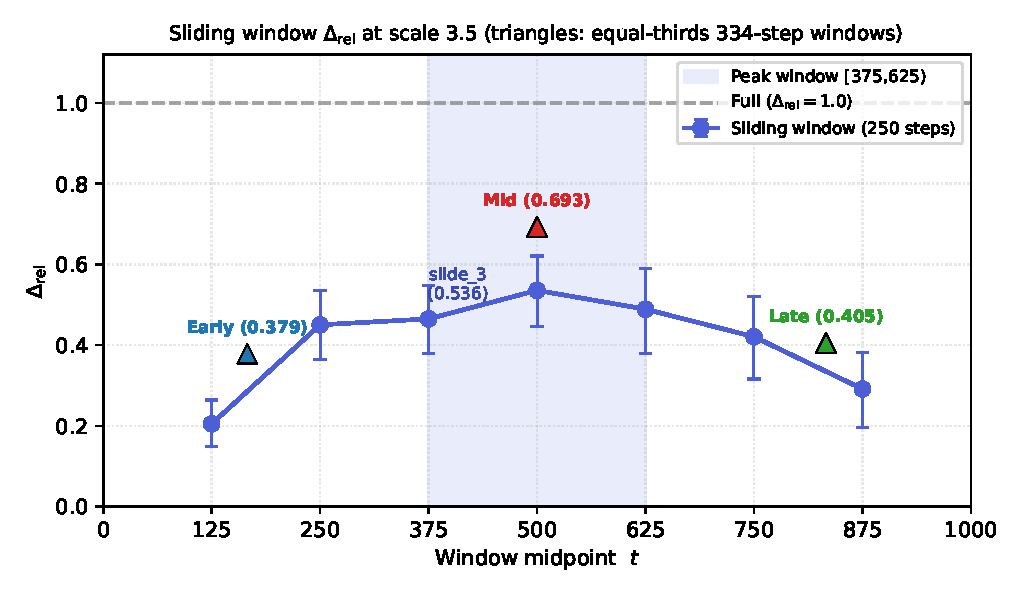
\includegraphics[width=0.82\linewidth]{fig2_sliding_window.pdf}
\caption{Sliding-window relative effect at $s=3.5$ (window width 250, step 125)
plotted against the window midpoint $t$.  The profile is unimodal with a peak
at \texttt{slide\_3} ($t\!\in\![375,625)$, midpoint $500$,
$\Delta_\mathrm{rel}=0.536$).  Triangles mark the original equal-thirds
early/mid/late reference windows.}
\label{fig:sliding}
\end{figure}

The peak window is centred at $t=500$ and lies fully inside the equal-thirds mid
range $[333,667)$ (the peak ends at $t=625$, $42$ steps before the mid/late
boundary), consistent with the mid-window dominance seen in the sweep.  The sliding windows are 250 raw timesteps wide,
whereas the equal-thirds mid window is 334 raw timesteps wide; accordingly the
sliding peak \texttt{slide\_3} ($t\!\in\![375,625)$) reaches
$\Delta_\mathrm{rel}=0.536$, lower than the 334-step equal-thirds mid window's
$\Delta_\mathrm{rel}=0.693$ at the same scale $s=3.5$.  This gap is consistent
with the narrower sliding width covering less of the receptive interval, not
with a contradiction or a different effective region.  As with
$\Delta_\mathrm{rel}$ elsewhere, this is an association across overlapping
windows, not a causal decomposition.

% -----------------------------------------------------------------------
\section{Results: Robustness}
\label{sec:robustness}

\paragraph{Sample-size sensitivity.}
The single-scale concern is the late-window result at $s=1.0$, which sits at the
Bonferroni boundary.  Recomputing the late-vs-baseline Wilcoxon test on the
first $n$ seeds in seed order: $p=0.113$ at $n=25$ (fails), $p=0.00665$ at
$n=35$ (passes $\alpha/7=0.00714$), and $p=0.00716$ at $n=50$ (fails).  The
result is fragile: it does not consolidate as $n$ increases from 35 to 50,
which is atypical of a true effect (which would be expected to strengthen or
hold as $n$ grows).  We treat the $s=1.0$ late result as genuinely marginal and
do not claim significance.  The mid and early windows pass at every
$n\in\{25,35,50\}$ for every scale, and from $s=2.0$ upward the late window
passes at every $n$.

\paragraph{Independent replication (seeds 51--100).}
We re-ran the five conditions at $s=3.5$ on independent seeds 51--100 (50 new
seeds).  The mid-window relative effect replicates closely: $\Delta_\mathrm{rel}
= 0.693$ on seeds 51--100, matching the $0.693$ obtained on seeds 1--50.  The
mid window again beats baseline on all 50 seeds ($W=0$, $r_\mathrm{rb}=1.000$,
$p<0.0001$), as does the early window ($W=0$, $r_\mathrm{rb}=1.000$), and the
late window remains significant ($W=65$, $p=3.13\times10^{-10}$,
$r_\mathrm{rb}=0.898$).  It is the mid finding specifically that replicates: the
mid relative effect is unchanged ($0.693\to0.693$), whereas the early and late
relative effects drift across the independent seed set (early $0.379\to0.334$,
late $0.405\to0.492$) and the underlying means shift (baseline $11.978\to12.759$,
mid $4.31\to4.60$).  The mid relative-effect match (0.693) thus reflects
similarly shifted numerator and denominator, not a literal absolute-effect
reproduction; the metric is also seed-set sensitive for the weaker (early, late)
windows.  We do not claim a full replication of the per-window effect sizes, only
that the mid-window relative effect reproduces tightly.

% -----------------------------------------------------------------------
\section{Discussion and Conclusion}
\label{sec:discussion}

Across the six-scale sweep the mid window has the largest single-window relative
effect at every scale; its lead over the late window is statistically significant
for $s\ge2.0$ (not at $s\le1.0$), and its relative effect rises with guidance
scale (Table~\ref{tab:crossscale}, Figure~\ref{fig:releffects}).  All three
windows produce detectable seed-wise effects at the operating scales,
contradicting strict binary localization: the early window beats baseline on all
50 seeds at every scale ($r_\mathrm{rb}=1.000$, $50/50$ wins), and the late
window---not significant for $s\le 1.0$---becomes significant from $s=2.0$
upward.  The sliding-window analysis at $s=3.5$ refines this picture: the
relative-effect profile is unimodal and peaks at the center of the chain
($t\!\in\![375,625)$, $\Delta_\mathrm{rel}=0.536$), consistent with mid-chain
dominance without a sharp boundary.

The cross-scale pattern---mid above early and late in point estimate at every
scale (the mid-vs-late gap significant for $s\ge2.0$), with early and late
statistically indistinguishable at every scale (late-vs-early never significant,
overlapping CIs)---is anchored on the
relative-effect numbers, not on intuition about diffusion dynamics.  We
emphasize that $\Delta_\mathrm{rel}$ uses $(\text{baseline}-\overline{\text{full}})$
as denominator; the full-chain \emph{mean loss} approaches $0$ as scale rises,
so the denominator \emph{grows} ($1.93$ at $s=0.5$ to $11.70$ at $s=7.0$).
This means ratio-estimator instability is worst at \emph{low} $s$ (where the
denominator is small and the late-window CI spans zero at $s=0.5$), not at high
$s$ as might be assumed.  The cross-scale comparison is still partly
denominator-sensitive and is an association, not a causal decomposition.

\textbf{Limitations}: single dataset (LSUN Bedroom), single architecture and
minority classifier, class 99, $n=1$ sample per seed; high variance that grows
with scale (full-chain CV $0.61$ at $s=1.0$ rising to $1.04$ at $s=7.0$, the mid
window reaching CV $1.49$ at $s=7.0$); no perceptual metrics (FID~\cite{heusel2017fid},
precision/recall).  The sweep adds two limitations.  First, pooling six scales
raises a cross-scale multiple-comparisons question: we correct within scale at
$\alpha/7=0.00714$ and note the stricter cross-scale threshold
$\alpha/42=0.00119$, under which the $s\le 1.0$ late-vs-baseline results remain
non-significant while the mid/early/full results and the $s\ge 2.0$ late results
continue to pass.  Second, the sweep remains a single dataset; scale generality
has been tested but dataset and architecture generality have not.  All six
scales, the cross-scale matrix, the sliding-window run, and the seeds 51--100
replication reproduce from their released raw CSVs.  The sliding-window analysis is a localization follow-up
to the sweep's mid-dominance pattern, and the seed-replication is a confirmatory
test of mid-window seed stability; the sample-size sweep is a post-hoc
robustness probe.  Each is Bonferroni-corrected within itself; we do not fold
their tests into a single study-wide family, and a stricter study-wide
correction would be more conservative still.

\textbf{Revised framing}: mid has the largest point-estimate relative effect at
every scale (statistically established vs.\ late for $s\ge2.0$; point-estimate
ordering only at $s\le1.0$) and the effect is distributed across windows; no
single equal-thirds window approximates full-chain performance, and the dominant
region is the center of the chain rather than a sharp early/late split.  The
case for treating the mid window as a cheaper inference-time guidance target is
most defensible at higher scales ($s\ge 3.5$), where the mid relative effect
reaches $0.693$--$0.832$ and replicates on independent seeds (the match reflects
similarly-shifted numerator and denominator, not literal absolute reproduction);
even there it recovers a fraction, not the whole, of the full-chain effect.

% -----------------------------------------------------------------------
\bibliographystyle{plain}
\bibliography{references}

% -----------------------------------------------------------------------
\appendix
\section{Reproducibility}
\label{sec:reproducibility}

\subsection{Experimental Configuration}
\label{sec:config}

\paragraph{Models and checkpoints} (all publicly available):

\begin{table}[h]
\centering
\caption{Model checkpoints used in all experiments.}
\renewcommand{\arraystretch}{1.1}
\begin{tabular}{@{}lll@{}}
\toprule
\textbf{Component} & \textbf{Checkpoint} & \textbf{Source} \\
\midrule
Diffusion model     & \texttt{lsun\_bedroom.pt}     & OpenAI guided-diffusion \\
Feature extractor   & \texttt{256x256\_classifier.pt} & OpenAI guided-diffusion \\
Minority classifier & \texttt{mc\_lsun.pt}          & Um et al.\ (2024) \\
\bottomrule
\end{tabular}
\end{table}

\paragraph{Shared hyperparameters} (all fixed across conditions; the
\texttt{guidance\_scale} column lists the six swept values):

\begin{table}[h]
\centering
\caption{Hyperparameters shared across all conditions and seeds.}
\renewcommand{\arraystretch}{1.1}
\begin{tabular}{@{}ll@{}}
\toprule
\textbf{Parameter} & \textbf{Value} \\
\midrule
\texttt{diffusion\_steps}       & 1000 \\
\texttt{timestep\_respacing}    & 250 \\
\texttt{noise\_schedule}        & linear \\
\texttt{guidance\_scale}        & 0.5, 1.0, 2.0, 3.5, 5.0, 7.0 (swept) \\
\texttt{image\_size}            & 256 \\
\texttt{num\_channels}          & 256 \\
\texttt{num\_res\_blocks}        & 2 \\
\texttt{attention\_resolutions} & 32,16,8 \\
\texttt{learn\_sigma}           & True \\
\texttt{use\_fp16}              & False \\
\texttt{manual\_class\_id}      & 99 \\
\texttt{num\_samples}           & 1 \\
\bottomrule
\end{tabular}
\end{table}

The minority classifier (\texttt{mc\_lsun.pt}) expects $8{\times}8$ latent features produced
by \texttt{256x256\_classifier.pt} with \texttt{pool=True}, \texttt{in\_channels=512},
\texttt{num\_channels=100}, \texttt{classifier\_width=128},
\texttt{classifier\_pool=attention}.

\textbf{unet.py patch}---the feature extractor
\texttt{256x256\_classifier.pt} loads as an \texttt{EncoderUNetModel}
(not the \texttt{UNetModel} used for diffusion sampling).  Its
\texttt{forward} is patched to expose the $8{\times}8$ pooled feature map:

\begin{lstlisting}[language=Python,caption={unet.py patch: expose intermediate pooled features during sampling.}]
def forward(self, x, timesteps, f_out=False):
    # skipping feature map extracted until final return
    if f_out:
        return h
    return self.out(h)  # original logic
\end{lstlisting}

\medskip
\noindent\textbf{Data schema} (one CSV per scale/experiment; one row per run):

\begin{center}
\small
\texttt{run\_id | condition | guidance\_window | t\_start | t\_end | guidance\_scale | seed | n\_generated | classifier\_mean\_confidence | classifier\_mean\_loss | runtime\_seconds | artifact\_path | timestamp}
\end{center}

\noindent Metrics are computed at \texttt{t=0} (final denoising step) by passing
generated images through the frozen classifier chain.  Each run
produces one image; \texttt{classifier\_mean\_\*} fields are single-sample
values (\texttt{n=1} per seed per condition).  The multi-scale sweep adds one
50-seed $\times$ 5-condition CSV per scale; the sliding-window run adds a
9-condition (baseline, full, \texttt{slide\_0}--\texttt{slide\_6}) CSV at
$s=3.5$; the replication run adds a 5-condition CSV for seeds 51--100 at $s=3.5$.
The sliding-window and seeds 51--100 replication runs share the configuration
above (the appendix model and hyperparameter tables) except for
\texttt{guidance\_scale}, the seed range, and the window boundaries.

% -----------------------------------------------------------------------
\subsection{Windowed Guidance Implementation}
\label{sec:implementation}

The windowed guidance requires no architectural modification---it is
implemented entirely within the \texttt{cond\_fn} callback:

\begin{lstlisting}[language=Python,caption={Windowed \texttt{cond\_fn}: applies classifier gradient only within [t\_start, t\_end).}]
t_start = args.t_start   # e.g. 333 for mid window
t_end   = args.t_end     # e.g. 667 for mid window

def cond_func(x, t=None):
    current_t = t[0].item()           # actual denoising timestep
    # Zero grad outside the active window
    if not (t_start <= current_t < t_end):
        return torch.zeros_like(x)
    with torch.enable_grad():
        x_in = x.detach().requires_grad_(True)
        latents   = f_extractor(x_in, timesteps=t, f_out=True)  # 8x8 pooled features
        logits    = classifier(latents, timesteps=t)            # minority classifier (mc_lsun.pt)
        log_probs = F.log_softmax(logits, dim=-1)
        selected  = log_probs[range(log_probs.shape[0]), y.view(-1)]
        # Scale applied only; sampler must NOT re-apply classifier_scale
        return torch.autograd.grad(selected.sum(), x_in)[0] \
               * args.classifier_scale
\end{lstlisting}

For baseline runs, \texttt{guidance\_scale=0} is passed rather than gating by
timestep.  Window boundaries are raw diffusion timesteps (0--1000); the active
window for mid is $t \in [333,667)$, corresponding to 334 of the 1000 raw
timesteps ($\approx\!83$ of the 250 respaced steps at stride 4).  The sliding-window run
uses a constant width of 250 raw timesteps stepped by 125.

% -----------------------------------------------------------------------
\subsection{Statistical Analysis Code}
\label{sec:stats}

\begin{lstlisting}[language=Python,caption={Statistical analysis: Wilcoxon signed-rank tests and rank-biserial correlation (n=50).}]
import csv, random
from scipy import stats

# --- load paired losses ---
data = {}
with open('data/multi_scale/runs_scale1p0_lsun_bedroom.csv') as f:  # schema identical across all scale CSVs
    for row in csv.DictReader(f):
        data.setdefault(row['condition'], {})[(int(row['seed']))] = \
            float(row['classifier_mean_loss'])

seeds = sorted(data['baseline'])
get   = lambda cond: [data[cond][s] for s in seeds]
baseline, early, mid, late, full = (get(c) for c in
    ['baseline','minority-early','minority-mid','minority-late','minority-full'])

# --- Wilcoxon signed-rank tests ---
def wilcoxon_rbc(a, b):
    diffs = [ai - bi for ai, bi in zip(a, b)]
    # zero_method='zsplit': split zero ranks equally between + and -
    W, p  = stats.wilcoxon(diffs, zero_method='zsplit')
    # rank-biserial: W / (n*(n+1)/2) * 2 - 1  (normalized to [0,1])
    n     = len(diffs)
    r_rb  = 1 - 2 * W / (n * (n + 1) / 2)
    return W, p, r_rb

comparisons = [
    (mid,   baseline, 'mid vs. baseline'),
    (late,  baseline, 'late vs. baseline'),
    (early, baseline, 'early vs. baseline'),
    (full,  baseline, 'full vs. baseline'),
    (mid,   late,     'mid vs. late'),
    (late,  early,    'late vs. early'),
    (full,  mid,      'full vs. mid'),
]

for a, b, label in comparisons:
    W, p, r_rb = wilcoxon_rbc(a, b)
    print(f'{label:<25}  W={W:>5.0f}  p={p:.4f}  r_rb={r_rb:.3f}')

alpha_corrected = 0.05 / 7  # = 0.00714 (per scale); cross-scale = 0.05/42 = 0.00119

# --- Bootstrap 95% CI on mid mean (10,000 resamples) ---
random.seed(42)
boot  = sorted([sum(random.choices(mid, k=50)) / 50  for _ in range(10_000)])
ci    = [boot[249], boot[9749]]  # 2.5th and 97.5th percentiles

baseline_mean  = sum(baseline) / len(baseline)  # 11.978
threshold      = 0.05 / 7                        # 0.00714
mid_mean       = sum(mid) / len(mid)             # 9.591 at s=1.0
\end{lstlisting}

\noindent\textbf{Bootstrap note.}  The code above computes the 95\% CI on the
mid \emph{mean loss} (Table~\ref{tab:crossscale} last column) via independent
resampling of mid losses (\texttt{random.seed(42)}, 10{,}000 resamples).  The
$\Delta_\mathrm{rel}$ error bars in Figure~\ref{fig:releffects} and
Figure~\ref{fig:sliding} use a different method: paired-seed resampling jointly
over (baseline, condition, full) losses, implemented via
\texttt{np.random.default\_rng(42)}, with output written to
\texttt{stats/results/delta\_rel\_cis.json} by \texttt{stats/make\_figures.py}.
These are two distinct quantities (absolute loss vs.\ relative effect) and use
two distinct bootstrap procedures; both use 10{,}000 resamples and seed 42.

\noindent\textbf{Environment}: Python 3.11, scipy 1.x, numpy 2.x.  All runs
generated on Kaggle (NVIDIA Tesla P100, float32, CUDA 11.x).

\noindent\textbf{Data availability}: All raw CSVs, stats scripts, and
reproducibility code are in the accompanying repository
(\url{https://github.com/VittoriaLanzo/windowed-minority-guidance-repro};
see \texttt{data/} subdirectory) and mirrored as a Kaggle dataset
(\url{https://www.kaggle.com/datasets/vittorialanzo/wmg-sweep-results}).
The Kaggle notebook that generated the runs is at
\url{https://www.kaggle.com/code/vittorialanzo/windowed-minority-guidance-extended}.
All three are currently private and will be made public on acceptance.

\end{document}
